\documentclass[11pt]{article}
\usepackage{natbib}
\usepackage{graphicx}
\usepackage{tikz}
\usetikzlibrary{shapes,arrows}
\usepackage{pdflscape}
\usepackage{hyperref}

% Default margins are too wide all the way around. I reset them here
\setlength{\topmargin}{-.5in}
\setlength{\textheight}{9in}
\setlength{\oddsidemargin}{.125in}
\setlength{\textwidth}{6.25in}
\setlength{\topmargin}{-.5in}
\setlength{\textheight}{9in}
\setlength{\oddsidemargin}{.125in}
\setlength{\textwidth}{6.25in} 

% Define block styles for the flow diagrams used in the document
\tikzstyle{decision} = [diamond, draw, fill=blue!20, 
    text width=4.5em, text badly centered, node distance=3cm, inner sep=0pt]
\tikzstyle{block} = [rectangle, draw, fill=blue!20, 
    text width=5em, text centered, rounded corners, minimum height=4em]
\tikzstyle{line} = [draw, -latex']
\tikzstyle{cloud} = [draw, ellipse,fill=red!20, node distance=3cm,
    minimum height=2em]



% Setting up title, etc 
\title{Filtering read alignments in BAM format} 
\author{Tonatiuh Pe\~{n}a-Centeno \\
University of Greifswald}
\date{\today}

 
\begin{document}  
\maketitle
\abstract{This note documents "filterBAM", a program designed to clean single and paired RNA-seq reads. 
The filter 
is based on filterPSL, a perl script written by Prof. Mario Stanke. Both filterPSL and filterBam are 
designed for the cleaning of data that will subsequently be applied to the gene prediction problem. 
Nevertheless, it should be possible to modify rather easily, if it is to be applied to a different type of 
application. filterBam is written in C++ and makes use of the Bamtools API \citet{barnett11:BamTools}.

\section{Introduction}
RNA-seq data has become an important source of information for tasks such as differential 
expression analysis and transcript quantification. Given that this new technology produces millions of 
such short-reads, bespoke methods and tools are required to process such big amounts of information. 
Furthermore, the introduction of the Sequence AlignMent Format (SAM) \citet{heng09:SAM} has meant that many  
alignment tools (Bowtie, GMAP, etc.) now produce outputs in such format or in its binary version, aka BAM.

filterBam is a C++ code that cleans alignment files in BAM format that is based on filterPSL, a Perl routine 
written by Prof. Dr. Mario Stanke for PSL files. filterPSL was mainly used as a preprocessing step for 
cleaning alignments obtained with e.g. BLAT. filterBam is supposed to supersede filterPSL by doing the same 
sort of preprocessing but on RNA-seq alignment data represented in BAM format. filterBAM includes the 
following filtering options:

\section{Main features}

\begin{table}
\begin{tabular} {|c|c|c|}
\multicolumn{3}{*}{All types of reads} \\ \hline
	& Screens out & unmapped alignments. \\
	& Screens out & alignments that do not comply with a pre-defined coverage level (default=80\%). \\
	& Screens out & alignments that do not comply with a pre-defined percentage of identity (default=92\%). \\
	& Screeens out & alignments whose insert gaps do not comply with a pre-defined distance (default=10). \\ \hline
\multicolumn{3}{*}{Single reads} \\ \hline
	& Screens out & groups of alignments that belong to a common query, if (best) \\ 
	& Screens out & groups of alignments that belong to a common query, if (unique) \\  
\multicolumn{3}{*}{Paired reads} \\ \hline
	& Screens out & paired alignments if (best) \\ 
	& Screens out & paired alignments if (uniq) \\
	& 
	& Writes to file & a prospective list of common target genes \\ 
	& Writes to file & a summary pairedness coverage. \\
\
\end{tabular}
\end{table}

The filter should work fine for filtering data coming from 454 and Illumina but not for SOLiD technology. 
The subsequent sections of this document describe how the filtering is done to single or paired-end reads.


\section{Single reads}
Operation of the single-read filter is described in a step by step basis because the paired-read filter works 
in a very similar way. Figure \ref{tik:singleReadFilter} below shows the schematics of the operation of 
the filter. Each read is processed independently, so assumming a set of reads $i\in {1,\dots,N}$, the 
filter processes independently each of them one at a time.

Firstly, the filter checks read $i$ is mapped or not. This is easily done by means of checking SAM field 
number 2, the alignment FLAG, and more specifically bit $0\times4$, which is the only source of reliable 
information to determine whether a read is mapped or not \citet{heng09:SAM}. This is achieved by using the 
$isMapped()$ methods of BamTools. Unmapped reads are dropped, while mapped reads continue further processing. A counter keeps track of the number of unmapped reads that were dropped. 

As a second step, reads that passed the mapping test are appended with two additional but temporary 
string-tags. Tag "co" and tag "pi" are added to the binary alignment by the $addTag()$ method of BamTools. 
"co" stands for \emph{coverage} and is a measure of the amount of reads located at a given genomic position. "pi" stands for \emph{percentage identity} and is a measure of the number of basis that correctly identify 
a genomic position. Estimation of the coverage is done according to Equation \ref{eq:coverage}, whilst estimation of the percentage identity is done following Equation \ref{eq:percId}. 

If the estimated coverage value for read $i$ is less than that of minCover, the read will be dropped and 
a counter keeping track of such types of drops will be updated. In a similar way, if the value of percId 
for read $i$, is less than that specified by minId, the read will be dropped and the corresponding counter 
will be updated. Default values for $minCover=80$ and $percId=92$ might be modified by using the options 
'--minCover <value>' and '--minId <value>'.

An optional value, the number of inserts to the base reference (baseInsert), is computed optionally if 
the '--noIntrons' option is used. The number of insertions to the reference is computed through the 
application of Equation \ref{eq:baseInsert}. This filter depends on the insertLimit value that has been 
specified, and which by default has a value of $10$. The insertLimit parameter might be modifed by 
applying the '--insertLimit <value>' option.

Once this filters have been applied: mapping filter, coverage filter, percentage identity filter and intron 
filter, a set of reads will be dropped out. From the remaining reads that satisfied such filter criteria, 
the information from coverage and percentage identity will be combined into a single figure, a \emph{score} 
that will help in determining which reads are worth keeping and which not.


\begin{figure}
  \centering
  \begin{tikzpicture}[node distance=2cm, auto]
    % Place nodes
    \node [cloud] (Start) {Start}; 
	\node [decision, below of=Start, node distance=3cm] (unmapped) {Unmapped reads};
    \node [block, below of=unmapped, node distance=3cm] (percId) {Compute percentage identity};
    \node [block, below of=percId, node distance=3cm] (coverage) {Compute coverage};
    \node [decision, below of=coverage, node distance=3cm] (noIntrons) {noIntrons?};
    \node [block, left of=noIntrons, node distance=3cm] (baseInsert) {Compute Insertions to the ref.};
    \node [block, below of=noIntrons, node distance=3cm] (unique) {Unique};
    \node [cloud, below of=unique, node distance=3cm] (End) {End};
    % Draw edges
    \path [line] (Start) -- (unmapped);
	%% \path [line] (unmapped -- node [near start] {yes} (percId);
    \path [line] (unmapped) -- node {no} (percId);
    \path [line] (percId) -- (coverage);
    \path [line] (coverage) -- (noIntrons);
    \path [line] (noIntrons) -- node [near start] {yes} (baseInsert);
    \path [line] (baseInsert) |- (unique);
    \path [line] (noIntrons) -- node {no}(unique);
    \path [line,dashed] (unique) -- (End);
  \end{tikzpicture}
  % Caption and label
  \caption{Flow diagram of the operation of the single-read filter}
  \label{tik:singleReadFilter}
\end{figure}


\subsection{Uniq and Best criteria}
Filtering by 'unique' or 'best' criteria is mutually exclusive, as Figure \ref{tik:singleReadFilter} shows. 
After passing the basic filtering scheme already described, all the remaining alignments that belong to 
a common query are scored through the function 

\begin{equation}
	\mathrm{score} = \mathrm{percId} + \mathrm{coverage}.
\end{equation}

The score is added as an optional tag to each alignment by means of the "addTag()" method of BamTools. 
Afterwards, this group of alignments is sorted by its scored value; as illustrated in Table 
\ref{tab:singleReads} below.

\begin{landscape}
  \centering
  \begin{table}
    \begin{tabular}{|l|l|l|l|}
      \hline
      r2/1	147	chr17	27698730	37	33M1I16M	=	27698611	-168	& Field10	& Field11	& XT:A:U	NM:i:1	SM:i:37	AM:i:0	X0:i:1	X1:i:0	XM:i:0	XO:i:1	XG:i:1	MD:Z:49 \\ \hline
      r2/1	99	chr17	20320141	36	43M1I6M	=	20320287	196	& Field10	& Field11	& 	XT:A:R	NM:i:3	SM:i:0	AM:i:0	X0:i:2	X1:i:0	XM:i:2	XO:i:1	XG:i:1	MD:Z:17C25A5 \\ \hline
      r2/1	99	chr19	1365	60	5M1I44M	=	8297	187	& Field10	& Field11	& 	XT:A:U	NM:i:1	SM:i:37	AM:i:37	X0:i:1	X1:i:0	XM:i:0	XO:i:1	XG:i:1	MD:Z:49 \\ \hline
      r2/1	83	chr17	8038459	60	45M1I4M	=	8038315	-193	& Field10	& Field11	& 	XT:A:U	NM:i:2	SM:i:37	AM:i:37	X0:i:1	X1:i:0	XM:i:1	XO:i:1	XG:i:1	MD:Z:21T27 \\ \hline
      r2/1	99	chr17	24524224	60	19M2I29M	=	24524392	218	& Field10	& Field11	& 	XT:A:U	NM:i:3	SM:i:37	AM:i:23	X0:i:1	X1:i:0	XM:i:1	XO:i:1	XG:i:2	MD:Z:11G36 \\ \hline
      r2/1	163	chr17	30676705	37	26M2I20M2S	=	30676860	205	& Field10	& Field11	& 	XT:A:M	NM:i:2	SM:i:37	AM:i:37	XM:i:0	XO:i:1	XG:i:2	MD:Z:46 \\ \hline
      r2/1	99	chr17	16894328	29	26M1I23M	=	16894487	209	& Field10	& Field11	& 	XT:A:R	NM:i:3	SM:i:0	AM:i:0	X0:i:4	X1:i:0	XM:i:2	XO:i:1	XG:i:1	MD:Z:4C1A42 \\ \hline
      r2/1	147	chr17	5031883	60	24M1I25M	=	5031761	-171	& Field10	& Field11	& 	XT:A:U	NM:i:2	SM:i:37	AM:i:37	X0:i:1	X1:i:0	XM:i:1	XO:i:1	XG:i:1	MD:Z:11A37 \\ \hline
      r2/1	83	chr18	1	0	10M1I39M	=	24	-206	& Field10	& Field11	& 	XT:A:R	NM:i:1	SM:i:0	AM:i:0	X0:i:2	X1:i:0	XM:i:0	XO:i:1	XG:i:1	MD:Z:49 \\ \hline
    \end{tabular}
    \caption{Some SAM alignments showing added tags: percId, coverage and score}
    \label{tab:singleReads}
  \end{table}
\end{landscape}

The difference between the 'unique' and 'best' criteria is that the former will select only the top-scored 
alignment and will write it into file. Table Y below shows the same set of alignments as in \ref{tab:singleReads} after ranking. According to the 'uniq' criterion, only the top-ranked alignmnent is elligible to be 
preserved. However, in case a group of alignments happen to share the same score, filterBam checks whether 
such alignments are similar. 

\subsection{Similarity function}

\begin{figure}
  \begin{center}
    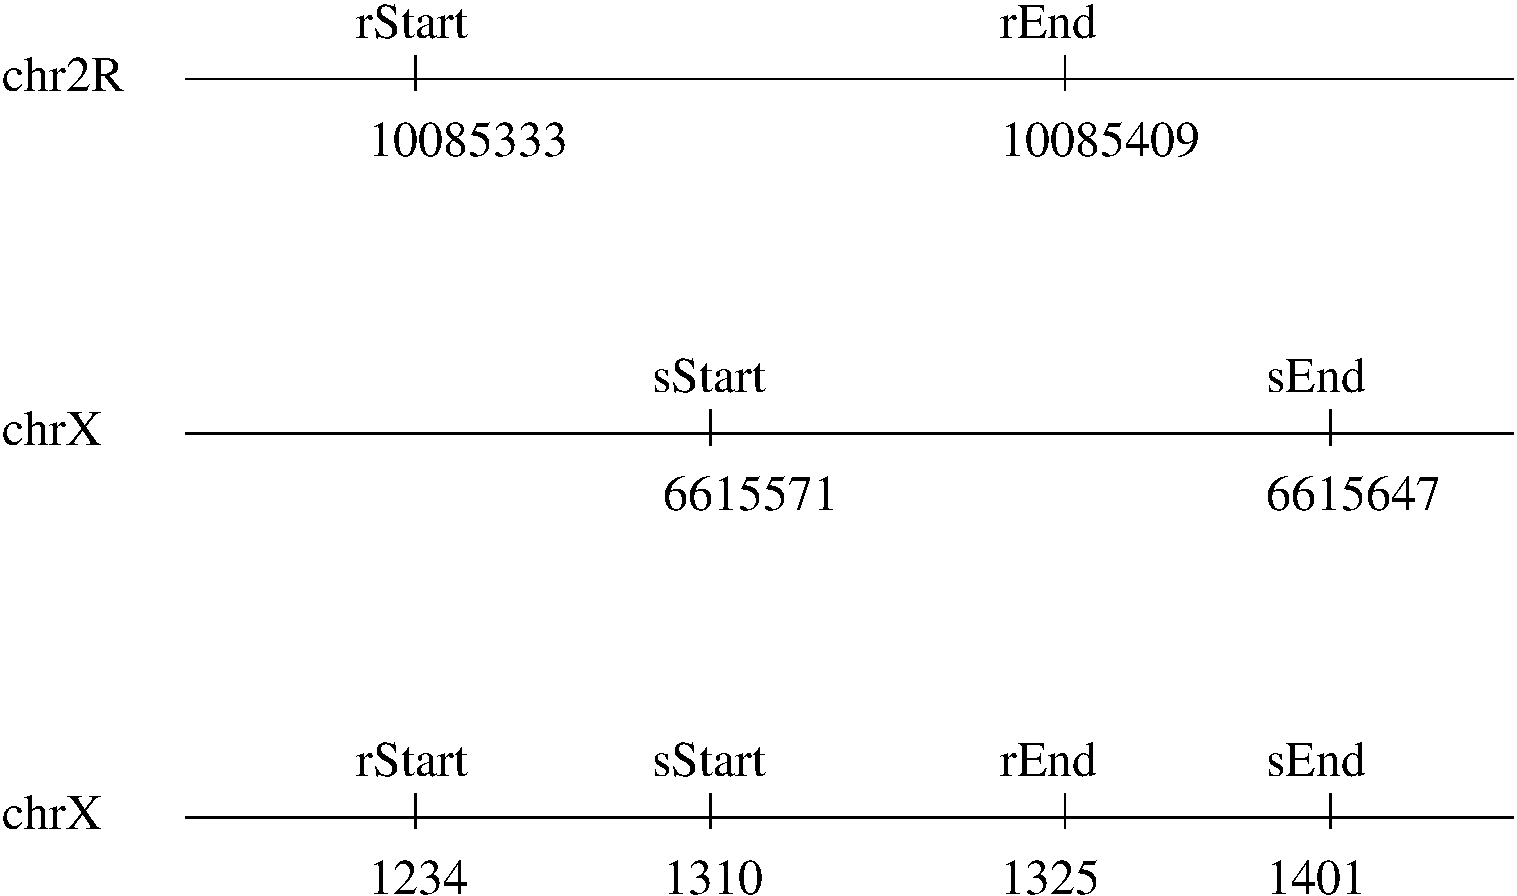
\includegraphics[width=7cm]{figures/similarFunction.pdf}
  \end{center}
\end{figure}



\section{Paired reads}

\begin{figure}
  \begin{center}
    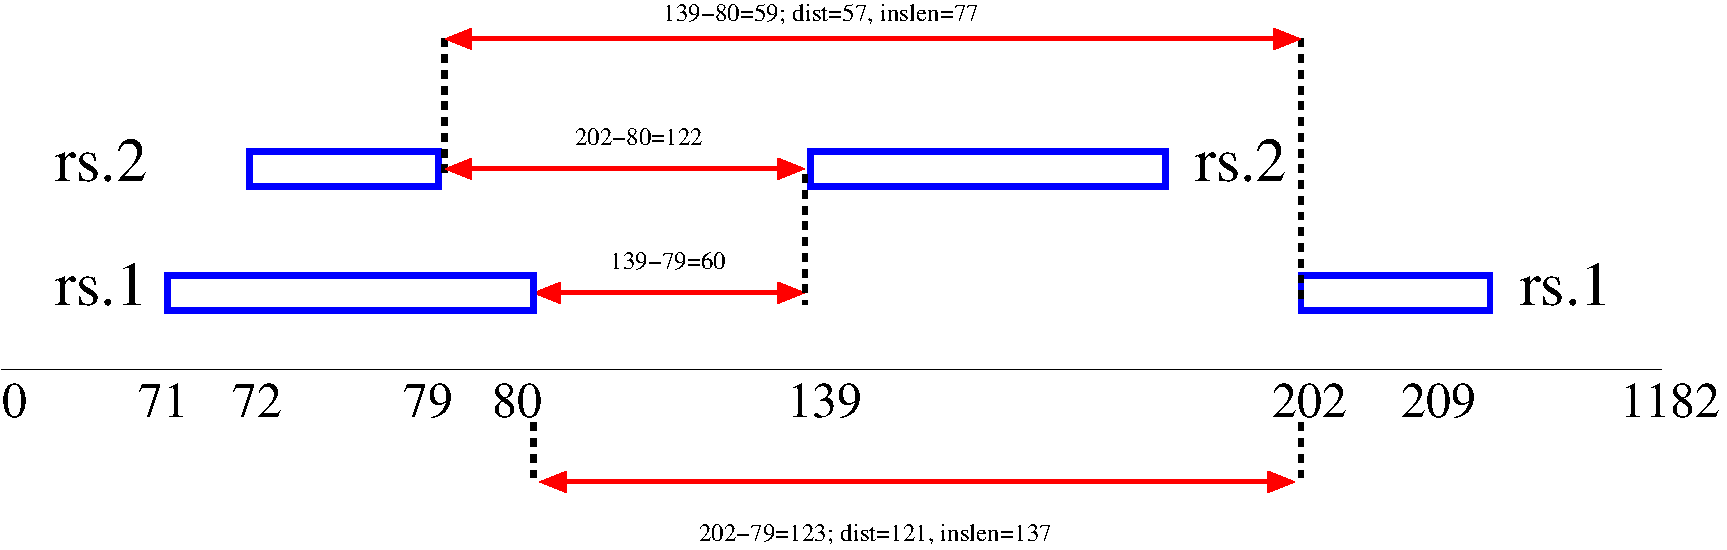
\includegraphics[width=7cm]{figures/pairedReads.pdf}
  \end{center}
\end{figure}


\section{Bamtools}
Bamtools is a C++ wrapper API of the more well-known Samtools software. The latest version of Bamools 
is 2.0 and is available on the website \url{https://github.com/pezmaster31/bamtools/downloads}. 

\section{Test data}
We have generated two data sets to show filterBam in operation. 

\section{Compilation}

Note that the flag ``-std=c++0'' has been used given that some of the functionalities of the filter require 
some of the newest features of GNU's g++ compiler. This and future versions of the software have been tested 
on Ubuntu's g++ version 4.4.3.

\section{How to run}
A run that will let pass most, if not all, readings: 
\begin{flushleft}
./filterBam input.bam output.bam --minCover 0 --minId 0  --insertLimit 10000000 --nointrons
\end{flushleft}
\textbf{Note:} that all options are provided at the very end.

Make sure to link with the ``-lz'' and ``-libbamtools.a'' flags on; where -lz refers to the ZLIB library, 
and libbamtools.a to the static bamtools library included in the software distribution. An example of 
how to compile and link follows: 

\begin{flushleft}
\begin{enumerate}
	\item	
		g++ -I\textbf{\$BAMTOOLS}/include   -g   -std=c++0x  -c filterBam.cc -o filterBam.o \\
	\item	g++     -g -std=c++0x  filterBam.o -o filterBam \textbf{\$BAMTOOLS}/lib/libbamtools.a -lz  
\end{enumerate}
\end{flushleft}
\vphantom{Nothing}
where \textbf{\$BAMTOOLS} is the path where Bamtools was installed.


\section{Coverage, percent of identity and insert length}
The coverage is computed as the sum of the alignment matches (sequence matches or mismatches) and 
the insertions to the reference. Both figures, alignment matches and insertions to the reference, correspond 
to CIGAR string operations $M$ and $I$, respectively. Thus the following is done 

\begin{equation}
	\mathrm{coverage} = \frac{\sum\mathrm{CIGAR}\left(M,I\right)}{qLength}
	\label{eq:coverage}
\end{equation}

An approximation to the percentage of identity is given by computing the query length and subtracting the 
so-called edit distance to the reference (tag ``NM'' in SAM jargon), i.e.

\begin{equation}
	\mathrm{percId} = \frac{qLength - \mathrm{Tag}(NM)}{qLength}
	\label{eq:percId}
\end{equation}

The length of inserts is estimated by summing CIGAR operations ``M'' and ``I'', which correspond to alingment 
matches and deletions from the reference. In other words, we do the following

\begin{equation}
	\mathrm{InsertSize} = \frac{\sum\mathrm{CIGAR}\left(D,I\right)}{qLength}
	\label{eq:baseInsert}
\end{equation}


\begin{thebibliography}{1}
\providecommand{\natexlab}[1]{#1}
\providecommand{\url}[1]{\texttt{#1}}
\expandafter\ifx\csname urlstyle\endcsname\relax
  \providecommand{\doi}[1]{doi: #1}\else
  \providecommand{\doi}{doi: \begingroup \urlstyle{rm}\Url}\fi

\bibitem[Li et~al.(2009)Li, Handsaker, Wysoker, Fennell, Ruan, Homer, Math,
  Abecasis, Durbin, and Subgroup]{heng09:SAM}
H.~Li, B.~Handsaker, A.~Wysoker, T.~Fennell, J.~Ruan, N.~Homer, G.~Math,
  G.~Abecasis, R.~Durbin, and .~G. P. D.~P. Subgroup.
\newblock The sequence alignment/map format and samtools.
\newblock \emph{Bioinformatics Applications Note}, 25\penalty0 (16):\penalty0
  2078--2079, 2009.

\bibitem[Barnett et~al.(2011)Barnett, Garrison, Quinlan, Strömberg and Marth]{barnett11:BamTools}
D.~Barnett, E.~Garrison, A.~Quinlan, M.~Strömberg, G.~Marth.
\newblock BamTools: a C++ API and toolkit for analyzing and managing BAM files.
\newblock \emph{Bioinformatics}, 27\penalty0 (12):\penalty0
  1691-1692, 2011.



\end{thebibliography}

%\bibliographystyle{abbrvnat}

\end{document}
